% TELOS Two-Layer Fidelity Pipeline
% Standalone compilable TikZ diagram
% Compile with: pdflatex fig3_fidelity_pipeline.tex

\documentclass[border=10pt]{standalone}
\usepackage{tikz}
\usetikzlibrary{positioning, arrows.meta}

\begin{document}
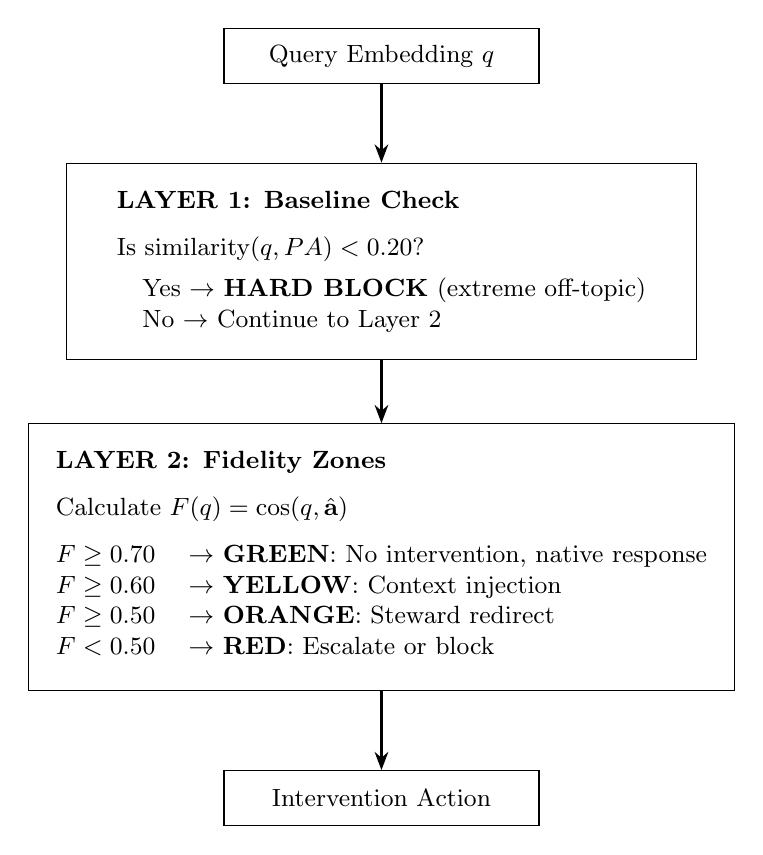
\begin{tikzpicture}[
    >=Stealth,
    node distance=0.8cm,
    box/.style={
        rectangle,
        draw,
        minimum width=8cm,
        align=left,
        inner sep=10pt,
        font=\small
    },
    smallbox/.style={
        rectangle,
        draw,
        minimum width=4cm,
        minimum height=0.7cm,
        align=center,
        font=\small
    },
    arrow/.style={->, thick}
]

% Input
\node[smallbox] (input) {Query Embedding $q$};

% Layer 1
\node[box, below=1cm of input] (layer1) {
    \textbf{LAYER 1: Baseline Check}\\[6pt]
    Is similarity$(q, PA) < 0.20$?\\[4pt]
    \hspace{1em}Yes $\rightarrow$ \textbf{HARD BLOCK} (extreme off-topic)\\
    \hspace{1em}No $\rightarrow$ Continue to Layer 2
};

% Layer 2
\node[box, below=0.8cm of layer1] (layer2) {
    \textbf{LAYER 2: Fidelity Zones}\\[6pt]
    Calculate $F(q) = \cos(q, \hat{\mathbf{a}})$\\[6pt]
    \begin{tabular}{@{}ll@{}}
    $F \geq 0.70$ & $\rightarrow$ \textbf{GREEN}: No intervention, native response\\
    $F \geq 0.60$ & $\rightarrow$ \textbf{YELLOW}: Context injection\\
    $F \geq 0.50$ & $\rightarrow$ \textbf{ORANGE}: Steward redirect\\
    $F < 0.50$ & $\rightarrow$ \textbf{RED}: Escalate or block\\
    \end{tabular}
};

% Output
\node[smallbox, below=1cm of layer2] (output) {Intervention Action};

% Arrows
\draw[arrow] (input) -- (layer1);
\draw[arrow] (layer1) -- (layer2);
\draw[arrow] (layer2) -- (output);

\end{tikzpicture}
\end{document}
